\chapter{Liver}
\label{sec:liver}
\label{chap:liver}

\section{Size}
\label{sec:liver-size}

The human adult liver weighs about 1.4 kg (3.1 pounds) 
\url{https://www.ncbi.nlm.nih.gov/pubmedhealth/PMH0072577/}


\section{Cells composition: lobules}
\label{sec:lobules}

Liver tissue is made up of lots of smaller units of liver cells called
{\bf lobules}.
Many canals carrying blood and bile run between the liver cells.

\section{Inputs}

Blood coming from the digestive organs flows through the portal vein to the
liver, carrying nutrients, medication and also toxic substances.


Once they reach the liver, these substances are processed, stored, altered,
detoxified, and passed back into the blood or released in the bowel to be
eliminated. In this way the liver can, for example, remove alcohol from your
blood and get rid of by-products from the breakdown of medications.


\section{Function}
\label{sec:liver-function}

\begin{enumerate}
  \item (with the help of vitamin K) liver produces proteins important for blood
  clotting
  
  \item break down oldd or damaged blood cells
  
  \item break down fats to produce energy: using bile
  
  \item produce bile: human liver produces 800 to 1,000 ml of bile per day.  
  
  This yellow, brownish or olive green liquid is collected in small ducts and
  then passed on to the main bile duct, which carries the bile to a part of the
  small intestine called the duodenum. Bile is important for the breakdown and
  absorption of fats.  

  \item regular blood sugar level:
  by converting excessive sugar into glycogen (Sect.\ref{sec:glycogen})
  
  \item  change amino acids in foods so that they can be used to produce energy,
  or make carbohydrates or fats
  
NOTE: This process creates a  toxic substance called ammonia as a by-product.

 The liver cells convert ammonia to a much less toxic substance called urea,
which is released into the blood. Urea is then transported to the kidneys and
passes out of the body in urine.
   
\end{enumerate}

\section{Intestine}
\label{sec:intestine}

The intestine involves into the process of food breakdown
(Sect.\ref{sec:stage-1}), and from here, small molecules are moved into the
bloodstream from tiny intestinal wall called {\bf villus}
(Sect.\ref{sec:villi}), Fig.\ref{fig:intestine-villus}.
It is the part of the digestive tract where approx 90\% of the digestion and
absorption of food occurs, the other 10\% taking place in the stomach and large
intestine.

\begin{figure}[htb]
  \centerline{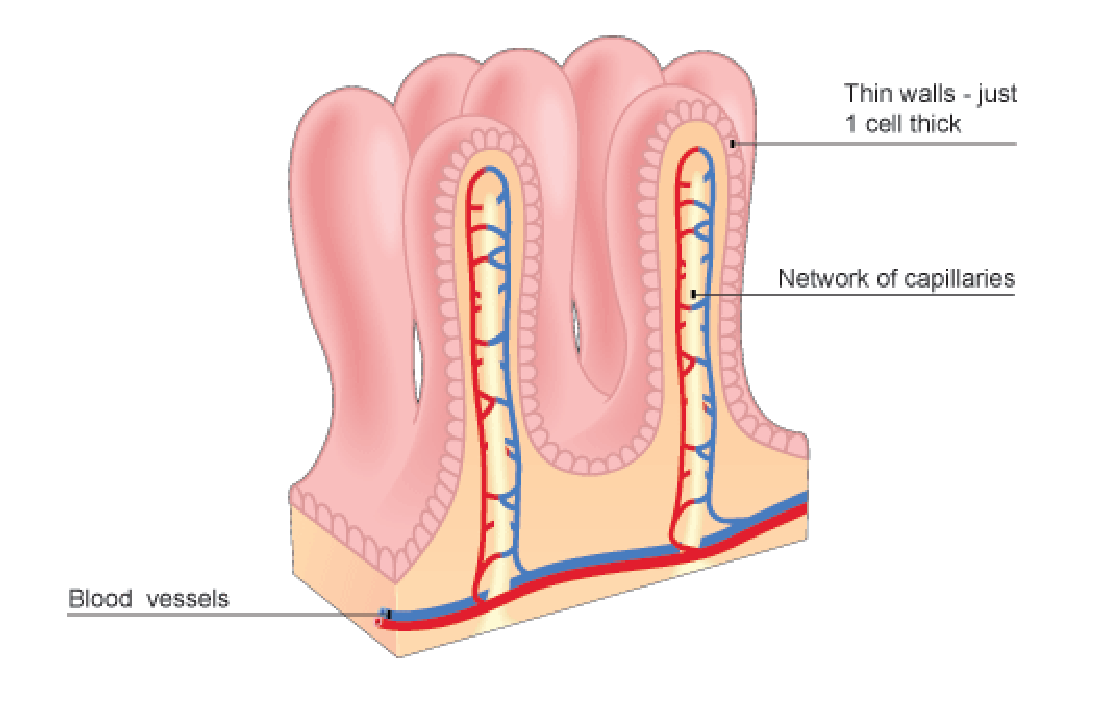
\includegraphics[height=3cm]{./images/intestine-villus.eps}}
  \caption{intestine's villus}
  \label{fig:intestine-villus}
\end{figure}


\subsection{-- passing into bloodstream}
\label{sec:villi-passing-small-molecules}

These are the molecules that can pass into the bloodstream (via different ways
as being described shortly)
\begin{enumerate}
  \item amino acids : breakdown from proteins
  
  Proteolytic enzymes e.g. including trypsin and chymotrypsin, secreted by the
  pancreas, break proteins into smaller peptides. (Chemical breakdown begins in
  the stomach and continues in the large intestine.) 
  
  \item fatty acids, and glycerol: breakdown from lipids (fats)
  
  Pancreatic lipase breaks triglycerides into free fatty acids and monoglycerides. 
It is helped by bile salts secreted by the liver and the gall bladder. They
attach to triglycerides, which aids access to the triglycerides by the
pancreatic lipase. This is because lipase is water-soluble but the fatty
triglycerides are hydrophobic so position themselves towards each other and away
from the watery intestinal surroundings. The bile salts hold the triglycerides
in the watery environment until the lipase can break them into the smaller parts
that can enter the villi for absorption.  

  \item simple sugars (e.g. glucose) - Sect.\ref{sec:monosaccharide}: breakdown
  from carbohydrates

Pancreatic amylase breaks down some carbohydrates, e.g. starch into
oligosaccharides.

Other carbohydrates pass undigested into the large intestine where they may,
depending on their type, be broken-down by intestinal bacteria.

\end{enumerate}


There are several ways for nutrient molecules to move across the villi to your
bloodstream: \textcolor{red}{simple/passive diffusion, facilitated diffusion,
primary active transport, or secondary active transport}, but the only nutrient
that moves by osmosis is water.

\subsection{---------by mechanisms}

Molecules are transported from the lumen of the small intestine into the
epithelial cells of the villi (inner-layer); then from those epithelial cells
into the underlying blood and lymphatic vessels in the submucosa
\begin{enumerate}
  \item {\bf passive/simple diffusion}: lipids, short-chain fatty acids
  
  \item {\bf facilitated diffusion}: fructose
  
  \item {\bf primary active transport}: amino acids  (primary or secondary
  active transport with Na+, followed by diffusion through the epithelial cells of the villus)
  
  \item {\bf secondary active transport}: Glucose (secondary active transport
  with Na+, followed by facilitated diffusion through the epithelial cells of the villus)
\end{enumerate}
This involves different mechanisms within the lumen of the small intestine vs.
through the epithelial tissue formed by the cells lining the villus.

\subsection{---------by molecules}

\begin{enumerate}
  \item {\bf monosaccharide}: 
  
  step 1 (from the lumen of small intestine into the epithelial cells of villi): 
  Glucose and galactose are transported by active transport. Fructose is
  transported by facilitated diffusion.
  
  step 2 (from inside of epithelial cells into bloodstream): by facilitated
  diffusion for all monosaccharide.
  
  \item {\bf amino acids, dipeptides, tripeptides}: 
  
  step 1: by  active transport processes - mainly in the duodenum and jejunum.
  
  step 2: by passive diffusion
  
  \item {\bf lipids (fats)}: 
  
  step 1 \& 2: by diffusion
  
  \item {\bf water}: absorbed by osmosis; with 80\% in small intestine and 10\%
  in large intestine; and 10\%  remaining excreted in the faeces.
  
Water moves across a permeable barrier during osmosis to equalize the solute
concentration on each side of the membrane.

  \item {\bf electrolytes}: Some electrolytes are from gastrointestinal
  secretions and others from ingested foodstuffs.
  
  \begin{itemize}
    \item sodium $\Na$: 
    
  step 1: by diffusion and active transport
  
  step 2: actively transported into blood capillaries on the other side of the
  epithelial cells.
  
    \item chloride ($\Cl$):
    
  step 1: can passively follow Na+ ions into epithelial cells, or be actively
  transported.
  
    \item  Ionide (\ce{I^-}): 
    
  step 1: can passively follow Na+ ions into epithelial
    cells, or be actively transported.
    
    \item Nitrate ($\ce{NO_3^-}$): can passively follow Na+ ions into epithelial
    cells, or be actively transported.
    
    \item Calcium $\Ca$: absorbed actively in a process stimulated by calcitriol
    (active form of Vitamin D).
    
    \item Iron ions (\ce{Fe^2+}, \ce{Fe^3+}): absorbed by active transport
    mechanisms
    
    \item Potassium $\K$: absorbed by active transport mechanisms.
    
    \item Magnesium $\Mg$: absorbed by active transport mechanisms.
    
    \item Phosphate ions $\ce{PO_4^{3-}}$: absorbed by active transport
    mechanisms.
  \end{itemize}

  \item {\bf vitamins}: 
  \begin{itemize}
    \item fat soluble vitamins (A, D, E and K) are absorbed together with
    dietary triglycerides.
    
    \item Most water-soluble vitamins (C and the B vitamins):  absorbed by
    diffusion.
    
    \item Vitamin B12 combined with intrinsic factor (from the stomach) is
    absorbed by active transport.
  \end{itemize}
\end{enumerate}


Some nutrients may be able to move across the barrier between the intestine and
blood with no help, others need a special structure to help them pass and a
third group require energy input to actively move them across the membrane. The
first two methods are known of as passive transport and the final is known as
active transport. 

The mechanism for passive transport is diffusion, where molecules move from an
area of higher concentration, the intestine, to an area of lower concentration,
the blood, through random movement.
\begin{enumerate} 
  \item Fats and fat soluble nutrients can move directly across the lipid
  membrane.
  
The end products of fat digestion, including glycerols, monoglycerides, and
fatty acids, are absorbed through diffusion directly across the cell membranes.


  \item Water, gasses, and other very small molecules can diffuse through the
  pores of the cell.  
  
  \item Larger molecules can move through specially designed channels made out
  of proteins.

Some larger particles are coated in bile salts, which allow them to pass through
the cell membrane.

Vitamin C and the B vitamins pass through protein channels using passive
diffusion. 

Fructose moves through facilitated diffusion, using a carrier protein to get
across the cell membrane. \textcolor{red}{Glucose, on the other hand, moves
through active transport (as it moves glucose against the concentration
gradient) and thus need ATP.} (Sect.\ref{sec:glucose-active-transport})
\end{enumerate}

  
\subsection{-- intestinal wall or intestinal villus (plural: villi)}
\label{sec:villi}
\label{sec:intestinal-wall}

The inside surfaces of small intestine have many folds called {\bf plicae
circulares}, from which project many tiny finger-like structures of tissue
called {\bf villi}, Fig.\ref{fig:intestine-villus}. The individual epithelial
cells also have finger-like projections, which are called known as {\bf
microvilli}. The functions of these all 3 structures: increase the surface area
available for the absorption of nutrients.

The inside wall of the small intestine needs to be thin (with only 2 layer of
cells), with a really big surface area. This allows absorption to happen quickly
and efficiently. If the small intestine had a thick wall and a small surface
area, a lot of digested food might pass out of the body before it had a chance
to be absorbed (Sect.\ref{sec:surface-volume-ratio}).

To get a big surface area, the inside wall of the small intestine is lined with
tiny villi (one of them is called a villus). These stick out and give a big
surface area. They also contain blood capillaries to carry away the absorbed
food molecules.

Each villus - made of many cells of 1 layer - is approximately 0.5-1.6 mm in
length (in humans), and has many microvilli projecting from the enterocytes of
its epithelium which collectively form the striated or brush border.
\begin{itemize} 

   \item Microvilli are microscopic cellular membrane protrusions, from a single
   cell in villus, that increase the surface area for diffusion and minimize any
   increase in volume.
 
   \item Thousands of microvilli form a structure called the brush border that
   is found on the apical surface of some epithelial cells, such as the small
   intestines. Not only for the function of villi, microvilli are also of
   importance on the cell surface of white blood cells, as they aid in the
   migration of white blood cells.

  \item  Though these are cellular extensions, there are little or no cellular
  organelles present in the microvilli.
  
  \url{https://en.wikipedia.org/wiki/Microvillus}
\end{itemize}

Villi are specialised for absorption in the small intestine as they have a thin
wall, {\bf one cell thick}, which enables a shorter diffusion path.  The villi
and the microvilli increase intestinal absorptive surface area approximately
30-fold and 600-fold, respectively.


\subsection{Glucose absorption: L-glucose active transport}
\label{sec:glucose-active-transport}

Notice: the active transport is between the inner of the intestine
into the cells on the wall of the villus. Then, from the cells to the
bloodstream is the passive process.
Mechanisms:
\begin{enumerate}
  \item  Sodium ions (Na+) are actively pumped out of the cells of the small
  intestine and into the blood via Sodium/Potassium (Na+/K+) pumps.
  
 The cells of the small intestine faces 2 sides: one side to the bloodstream,
 and the other side to the lumen of small intestines.
  
  \item  This creates an Na+ concentration gradient, where there is a higher
  concentration of Na+ in the lumen of the small intestine than inside the cells.
  
  \item  The Na+ then re-enters the cells of the small intestine via diffusion
  through a sodium-glucose transporter protein (alongside glucose).
  
So, for every sodium molecule get into cells, glucose also get co-transport into
the cells. From the cells, then glucose can get into the bloodstream.
  
  \item The glucose concentration inside the cell increases and a concentration
  gradient is created between the inside of the cells and the blood. This allows
  glucose to move via facilitated diffusion into the blood.  
\end{enumerate}
\url{https://www.mytutor.co.uk/answers/6406/A-Level/Biology/What-is-active-transport-and-how-is-it-used-in-the-absorption-of-glucose}

In the early studies:
\begin{itemize}
  \item It seems probable that L-glucose active transport is mediated by the mechanism
that actively transports D-glucose (Sect.\ref{sec:D-and-L-form}).

The L-glucose active transport was independent of net water movement, needed
oxygen, and required Na ions at a concentration of 83 mM or greater. It could be
completely inhibited by 10 $\muM$ phlorrhizin, or 10 mM l-histidine, or 1.39 mM
d-glucose.

Phlorrhizin at a concentration of 0.01 $\muM$ reduced, but did not prevent,
l-glucose active transport.
\url{https://www.ncbi.nlm.nih.gov/pmc/articles/PMC1365284/}
\end{itemize}


\section{Esophagys}
\label{sec:esophagys}  

Esophagys is a long (about 25cm), thin (2cm diameter), muscular tube that
connects the pharynx (i.e. throat) to the stomach (Sect.\ref{sec:stomach}). The
esophagus connects to the stomach at a small region called the cardia. The
cardia empties into the body of the stomach, which forms the central and largest
region of the stomach.

\section{Stomach}
\label{sec:stomach}  

The stomach is a hollow organ, or "container," that holds food while it is being
mixed with acid, mucus, and enzymes that continue the process of breaking down
food into a usable form (Sect.\ref{sec:stage-1}).
\begin{itemize}
  \item Superior to the body is a dome shaped region known as the fundus.
  \item Inferior to the body is a funnel shaped region known as the pylorus. 
  
  The pylorus connects the stomach to the {\it duodenum} and contains the
  pyloric sphincter. The pyloric sphincter controls the flow of partially digested food
  (known as {\bf chyme}) out of the stomach and into the duodenum.
  
\end{itemize}

The inner of the stomach is full of wrinkles known as {\bf rugae} (gastric
folds). Cells in the lining of the stomach secrete a strong acid and powerful
enzymes that are responsible for the breakdown process. When the contents of the
stomach are sufficiently processed (into {\bf chyme}), they are released into
the small intestine.

Digestion in the stomach can be divided into 2 classes: mechanical digestion and
chemical digestion. Mechanical digestion is the physical division of a mass of
food into smaller masses while chemical digestion is the chemical conversion of
larger molecules into smaller molecules.   

The smooth muscles of the stomach produce contractions known as mixing waves
that mix the boluses of food with gastric juice. This mixing leads to the
production of the thick liquid known as chyme. 

While food is being physically mixed with gastric juice to produce chyme, the
enzymes present in the gastric juice chemically digest large molecules into
their smaller subunits. 

\begin{enumerate}
  \item  Gastric lipase splits triglyceride fats into fatty acids and
  diglycerides. 

Gastrin, produced by the G cells of the stomach itself, increases the activity
of the stomach by stimulating increased gastric juice production, muscle
contraction, and gastric emptying through the pyloric sphincter. 
  
  \item Enzyme Pepsin breaks proteins into smaller amino acids.
  
  \item Cholecystokinin (CCK), produced by the mucosa of the duodenum, is a
  hormone that acts to slow gastric emptying by contracting the pyloric
  sphincter. 
  
  CCK is released in response to food rich in proteins and fats, which are
  difficult for the body to digest. By inhibiting gastric emptying, CCK allows
  food to be stored in the stomach longer to promote improved digestion by the
  stomach and to give the pancreas and gallbladder time to release enzymes and
  bile to increase digestion in the duodenum.
  
  The release of bile by CCK also helps neutralizing the acidic effect by chyme.
  
  \item  Secretin also promotes the production of pancreatic juice and bile that
  contain acid-neutralizing bicarbonate ions. The net effect of secretin is to
  protect the intestines from the damaging effects of acidic chyme. 
  
Secretin, another hormone produced by the duodenum's mucosa, responds to the
acidity of chyme entering the duodenum from the stomach. Secretin travels
through the bloodstream to the stomach where it slows the production of gastric
juice by the exocrine glands of the mucosa  
\end{enumerate}
\url{http://www.innerbody.com/image_digeov/dige11-new.html}
